%\documentclass[11pt,a4paper]{article}
%\usepackage{fullpage}
%\usepackage{beamerarticle}
%\documentclass[handout,xcolor=pdftex,dvipsnames,table]{beamer}
\documentclass[hyperref={unicode=true}]{beamer}

%\usepackage{pgfpages} 
%\pgfpagesuselayout{resize}[a4paper,border shrink=5mm,landscape] 

\usepackage[utf8]{inputenc}
\usepackage[russian]{babel}
\usepackage{../clrscode3e} 
\usepackage[all]{xy}
\usepackage{colortbl}
\usepackage{xcolor}
%\usepackage{pstricks, pst-tree, pst-node}
\usepackage{epsfig}
\usepackage{multicol}

\definecolor{orange}{cmyk}{0,0.52,1,0}

%\usepackage{beamerthemesplit}

\AtBeginSubsection[]
{
  \begin{frame}<beamer>{Раздел}
    \tableofcontents[currentsection,currentsubsection]
  \end{frame}
}


\newtheorem{rtheorem}{Теорема} 
%default}
%themesplit}

\title{B-деревья}
\subtitle{Дискретный анализ 2012/13}
\author{Андрей Калинин, Татьяна Романова}
\date{17 сентября 2012\,г. }
\usetheme{default}
%\usefonttheme{serif}
\usefonttheme[onlymath]{serif}
%\usefonttheme{professionalfonts}
%\usetheme{default} 


\begin{document}

\frame{\titlepage}

%\section[Содержание]{}
\frame{\tableofcontents}

%\section{Литература}
\frame
{
  \frametitle{Литература}

  \begin{itemize}
  \item  Кормен Т., Лейзерсон Ч., Ривест Р., Штайн К.. Алгоритмы:
    построение и анализ, 2-е издание, М.:Вильямс, 2005, стр. 515-536, глава 18,
    <<B-деревья>>. 
  \item  Кнут Д. Искусство программирования, Т.3: Сортировка и поиск,
    стр. 516-526, глава 6.2.4, <<Сильноветвящиеся деревья>>.
  \end{itemize}
}

\section{Определение B-дерева}
\subsection{Общая идея}
\frame
{
  \frametitle{Мотивация}
  \begin{itemize}
    \item Данные (и ключи) могут не помещаться в оперативную память. 
    \item Нужно иметь простой механизм загрузки нужной информации. 
    \item Для деревьев просто загружать и выгружать узлы, но у
      двоичных деревьев в узлах хранится слишком мало информации,
      чтобы работа с внешнией памятью была бы эффективна (слишком
      частые обращения неприемлимы). 
    \item Нужны сбалансированные деревья с большой степенью ветвления,
      в узлах которых хранилось бы много данных, тысячи ключей.  
  \end{itemize}
}

\frame{
  \frametitle{Пример B-дерева}
\includegraphics[scale=1]{b-tree.13.eps}
}

\frame{
  \frametitle{Размер B-дерева}
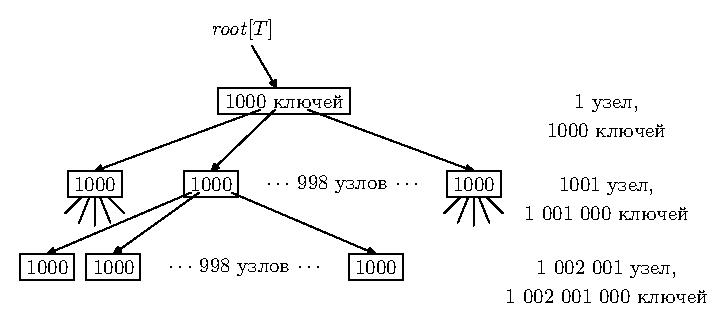
\includegraphics[scale=1]{b-tree.2.eps}
  
}

\frame
{
  \frametitle{Нестрогое понятие B-дерева}
  
  B-дерево степени $t$:
  \begin{itemize}
    \item Идеально сбалансированно. 
    \item Во всех узлах хранится до $2t-1$ ключей и $2t$
      соответствующих им указателей на поддеревья. 
    \item Во всех узлах, кроме корневого, хранится как минимум $t-1$
      ключей. В корневом узле хранится как минимум 1 ключ. 
    \item Ключи в узлах отсортированы. 
    \item В поддереве, расположенным между двумя последовательными
      ключами, находятся значения, большие первого и меньшие второго
      значения этих ключей. 
  \end{itemize}
}

\subsection{Определение}
\frame
{
  \frametitle{Определение B-дерева}
  B-дерево $T$ представляет из себя корневое дерево с корнем
  $\id{root}[T]$.

  Каждый узел $x$ дерева $T$ содержит следующие поля:
  \begin{enumerate}
    \item $n[x]$, количество ключей в $x$.
    \item $n[x]$ ключей: $\id{key}_1[x] \leq \id{key}_2[x] \leq \cdots \leq
      \id{key}_{n[x]}[x]$.
      \item Признак листа, $\id{leaf}[x]$.
      \item Внутренние узлы содержат $n[x]+1$ указателей на поддеревья: $c_1[x]$, $c_2[x]$,
        \ldots , $c_{n[x]+1}[x]$. Листья таких указателей не
        содержат. 
  \end{enumerate}
}

\frame{
  \frametitle{Определение B-дерева}
  \begin{itemize}
    \item Ключи $\id{key}_i[x]$ определяют диапазоны ключей в
      поддеревьях. Если $k_i$ --- произвольный ключ из поддерева
      $c_i$, то: $k_1 \leq key_1[x] \leq k_2 \leq \id{key}_2[x] \leq
      \cdots \leq \id{key}_{n[x]}[x] \leq k_{n+1}$.
    \item Все листья расположены на одной и той же высоте, $h$.
    \item $t$: минимальная степень B-дерева. 
    \item Каждый узел, кроме корневого, может содержать как минимум
      $t-1$ ключ. Корневой узел непустого дерева должен содержать как
      минимум 1 ключ. 
    \item Каждый узел не может содержать больше $2t-1$ ключей. 
  \end{itemize}
}

\subsection{Минимальная высота B-дерева}
\frame{
  \frametitle{Минимально заполненное B-дерево}
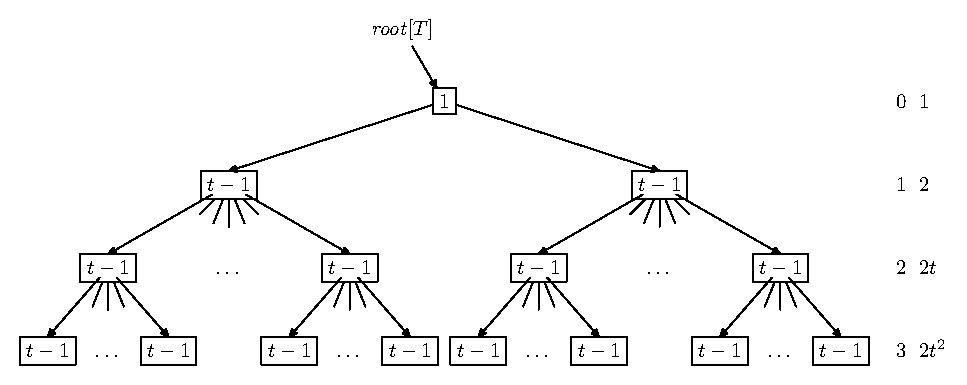
\includegraphics[scale=.7]{b-tree.3.eps}
}

\frame{
  \frametitle{Минимальная высота B-дерева}
  \begin{rtheorem}
    Высота B-дерева $T$ с $n \geq 1$ ключами и минимальной степенью~$t$
    не превышает $\log_t(n+1)/2$.
  \end{rtheorem}
  \begin{proof}
    \[
    n \geq 1 + (t-1)\sum_{i=1}^{h}2t^{i-1}=1+2(t-1)\frac{t^h-1}{t-1} =
    2t^h -1,
    \]
    откуда $t^h \leq (n+1)/2$.
  \end{proof}
}

\section{Операции с B-деревом}

\subsection{Создание}

\frame{
  \frametitle{Операции доступа к внешней памяти}
  \begin{itemize}
    \item $\proc{Disk-Read}(\id{node})$ --- чтение данных из внешней
      памяти в узел. 
    \item $\proc{Disk-Write}(\id{node})$ --- запись данных из узла во
      внешнюю память. 
    \item Конкретная реализация подразумевает наличие LRU (last recent
      used) буфера некоторого размера, при которой все часто
      используемые узлы остаются в памяти. 
      \item В алгоритмах предполагается, что корневой узел всегда
        находится в памяти, хотя на практике это необязательно: при
        LRU-буферизации корневой узел будет всегда
        оставаться в памяти и так. 
  \end{itemize}
}

\frame{
  \frametitle{Создание B-дерева}
  \begin{codebox}
    \Procname{$\proc{BTree-Create}(T)$}
    \li $x \gets \proc{Allocate-Node}()$
    \li $\id{leaf[x]} \gets \const{True}$
    \li $n[x] \gets 0$
    \li $\proc{Disk-Write(x)}$
    \li $\id{root}[T] \gets x$
    \End
  \end{codebox}
}

\subsection{Поиск}

\frame{
  \frametitle{Поиск в B-дереве}
  \begin{codebox}
    \Procname{$\proc{BTree-Search}(x,k)$}
    \li $i \gets 1$
    \li \While  $i \leq n[x]$ \func{and} $k>\id{key}_i[x]$
    \li \Do $i \gets i + 1$ \End
    \li \If $i \leq n[x]$ \func{and} $k \isequal \id{key}_i[x]$
    \li \Then \Return $(x,i)$ \End
    \li \If $\id{leaf}[x]$
    \li \Then \Return $\const{nil}$
    \zi \Else 
    \li $\proc{Disk-Read}(c_i[x])$
    \li \Return $\proc{BTree-Search}(c_i[x],k)$
    \End
  \end{codebox}
}

\subsection{Вставка}

\frame{
  \frametitle{Общая идея}
  \begin{itemize}
    \item Ищется лист, в который можно вставить новый ключ. 
    \item Нельзя просто так создать новый лист: в листьях должно быть
      как минимум $t-1$ ключей. 
    \item Заполненные узлы разбиваются на два по медиане: медиана
      уходит в родительский узел, вторая половинка существующего узла
      становится новым узлом. 
    \item Для вставки за один проход при поиске листа разбиваются все
      заполненные узлы вне зависимости от того, было ли это необходимо
      или нет. 
  \end{itemize}
}

\frame{
  \frametitle{Разбиение узла, $t=4$}
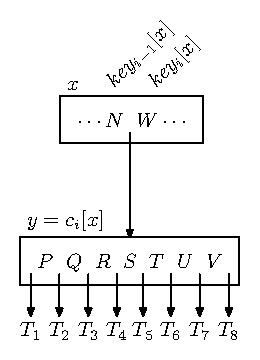
\includegraphics[scale=1]{b-tree.4.eps}\hfill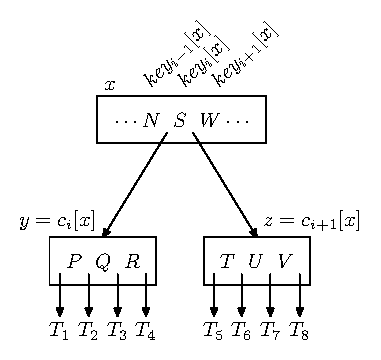
\includegraphics[scale=1]{b-tree.5.eps}
}

\frame{
  \frametitle{Разбиение узла B-дерева}
  \begin{multicols}{2}
  \begin{codebox}
    \Procname{$\proc{BTree-Split-Child}(x,i,y)$}
    \li $z \gets \proc{Allocate-Node}()$
    \li $\id{leaf}[z] \gets \id{leaf}[y]$
    \li $n[z] \gets t-1$
    \li \For $j \gets 1$ \To $t-1$
    \li   \Do $\id{key}_j[z] \gets \id{key}_{j+t}[y]$ \End
    \li \If \func{not} $\id{leaf}[y]$
    \li   \Then \For $j \gets 1$ \To $t$
    \li   \Do $c_j[z] \gets c_{j+1}[y]$ \End \End
    \li $n[y] \gets t-1$
    \li \For $j\gets n[x]$ \Downto $i+1$
    \li   \Do $c_{j+1}[x]\gets c_j[x]$ \End
    \end{codebox}
    \begin{codebox}
    \setcounter{codelinenumber}{11}
    \li $c_{j+1} \gets z$
    \li \For $j \gets n[x]$ \Downto $i$
    \li   \Do $\id{key}_{j+1}[z] \gets \id{key}_j[x]$ \End
    \li $\id{key}_i[x] \gets \id{key}_t[y]$
    \li $n[x] \gets n[x]+1$
    \li $\proc{Disk-Write}(y)$
    \li $\proc{Disk-Write}(z)$
    \li $\proc{Disk-Write}(x)$
    \End
  \end{codebox}
  \end{multicols}
}

\frame{
  \frametitle{Вставка ключа $k$ в B-дерево}
  \begin{codebox}
    \Procname{$\proc{BTree-Insert}(T,k)$}
    \li $r \gets \id{root}[T]$
    \li \If $n[r] \isequal  2t -1$
    \li   \Then $s \gets \proc{Allocate-Node}()$
    \li      $\id{root}[T] \gets s$
    \li      $\id{leaf}[s] \gets \const{false}$
    \li      $n[s] \gets 0$
    \li      $c_1[s] \gets r$
    \li      $\proc{BTree-Split-Child}(s,1,r)$
    \li      $\proc{BTree-Insert-Nonfull}(s,k)$
    \zi    \Else 
    \li $\proc{BTree-Insert-Nonfull}(r,k)$
  \end{codebox}
}

\frame{
  \frametitle{Разбиение корня, $t=4$}
\hfill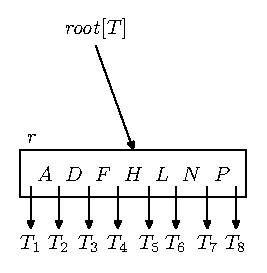
\includegraphics[scale=1]{b-tree.6.eps}\hfill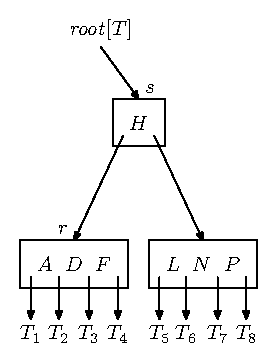
\includegraphics[scale=1]{b-tree.7.eps}\hfill~
}

\frame{
  \frametitle{Вставка ключа $k$ в незаполненный узел $x$}
%  \begin{multicols}{2}
    %\begin{column}
      \begin{codebox}
%        \def\codeindent{\textbf{el} }
        \Procname{$\proc{BTree-Insert-Nonfull}(x,k)$}
        \li $i \gets n[x]$
        \li \If $\id{leaf}[x]$ 
        \li     \Then \While $i \geq 1$ \func{and} $k < \id{key}_i[x]$ 
        \li           \Do $\id{key}_{i+1}[x] \gets \id{key}_i[x]$ ; 
                       $i \gets i - 1$ \End
        \li           $\id{key}_{i+1}[x] \gets k$ ; 
                   $n[x] \gets n[x] + 1$
        \li           $\proc{Disk-Write}(x)$
%      \end{codebox}
    %\end{column}
    %\begin{column}
%      \begin{codebox}
%        \def\codeindent{\textbf{el} }
%        \setcounter{codelinenumber}{8}
        %\Indentmore
         \li    \Else 
         \While $i\geq 1$ \func{and} $k < \id{key}_i[x]$
        \li           \Do $i \gets i - 1$ \End
        \li            $i \gets i+1$
        \li            $\proc{Disk-Read}(c_i[x])$
        \li            \If $n[c_i[x]] \isequal 2t-1$
        \li              \Then $\proc{BTree-Split-Child}$
        $(x,i,c_i[x])$
        \li                    \If $k>\id{key}_i[x]$
        \li                       \Then $i\gets i+1$ \End \End
        \li            $\proc{BTree-Insert-Nonfull}$
        $(c_i[x],k)$
        \End
      \end{codebox}
    %\end{column}
%  \end{multicols}
}


\frame{
  \frametitle{Исходное дерево}
\begin{center}
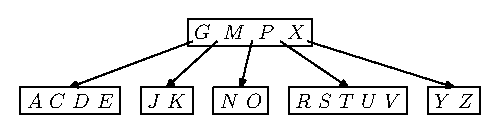
\includegraphics[scale=1]{b-tree.8.eps}
\end{center}
}

\frame{
  \frametitle{Вставка $B$}
\begin{center}
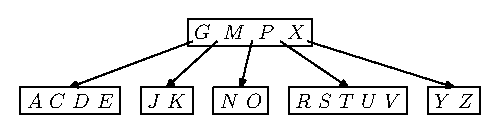
\includegraphics[scale=1]{b-tree.8.eps}\\
~\\
~\\
~\\
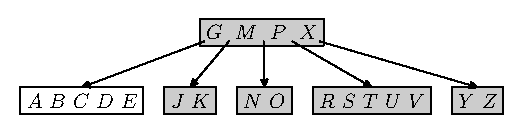
\includegraphics[scale=1]{b-tree.9.eps}
\end{center}
}

\frame{
  \frametitle{Вставка $Q$}
\begin{center}
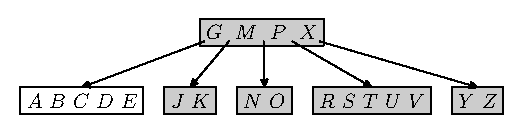
\includegraphics[scale=1]{b-tree.9.eps}\\
~\\
~\\
~\\
\includegraphics[scale=1]{b-tree.10.eps}
\end{center}
}

\frame{
  \frametitle{Вставка $L$}
\begin{center}
\includegraphics[scale=1]{b-tree.10.eps} \\
~\\
~\\
~\\
\includegraphics[scale=1]{b-tree.11.eps}
\end{center}
}

\frame{
  \frametitle{Вставка $F$}
\begin{center}
\includegraphics[scale=1]{b-tree.11.eps}\\
~\\
~\\
~\\
\includegraphics[scale=1]{b-tree.12.eps}
\end{center}
}

\subsection{Удаление}

\frame{
  \frametitle{Общая идея}
  \begin{itemize}
    \item В общем аналогично вставке, но вместо разбиения узлов они
      либо сливаются, либо используется <<перетекание>> ключей из
      соседних узлов через родительский. 
    \item Однако, технически более сложное: ключ может быть удалён
      откуда угодно, не только из листьев. 
    \item Нужно обеспечить, чтобы везде на пути были бы узлы, из
      которых при необходимости можно удалить ключ, т.е. минимальное
      количество ключей $t$. 
  \end{itemize}
}

\frame{
  \frametitle{Удаление ключа $k$}
  При проходе дерева могут возникнуть следующие три случая:
  \begin{enumerate}
  \item Если ключ $k$ находится в узле $x$ и $x$ --- лист, то удаляем $k$ из
    $x$. 
  \item Ключ $k$ находится в узле $x$ и $x$ --- внутренний узел:
    необходимо найти предшествующий или следующий ключ $k'$, удалить
    его и заменить $k$ в узле $x$ на $k'$.
  \item Ключ $k$ отсутствует во внутреннем узле $x$, то находим
    корень поддерева $c_i[k]$, в котором находится ключ $k$ и
    удостоверяемся, что он содержит как минимум $t$ ключей. В
    противном случае модифицируем дерево таким образом, чтобы в узле
    $c_i[k]$ было бы $t$ ключей. 
  \end{enumerate}
}

\frame{
  \frametitle{Второй случай}
  Узлы $y$ и $z$ --- дочерние по отношению к $x$, один предшествует
  ключу $k$, другой --- следует за ним. 
  \begin{itemize}
    \item $y$ содержит как минимум $t$ ключей, то находим $k'$ ---
      предшественника $k$ в поддереве $y$, удаляем его и заменяем его
      значением позицию ключа $k$ в $x$.
    \item Симметричная ситуация в $z$.
    \item $x$ и $y$ содержат по $t-1$ ключу: вносим $k$ и все ключи $z$
      в $y$, освобождаем $z$, удаляем $k$ из $y$. 
  \end{itemize}
}

\frame{
  \frametitle{Третий случай}
  Узел $c_i[x]$ --- корень поддерева, сдержащего $k$. Если в нём
  содержатся $t-1$ ключей, выполняем одно из следующих действий:
  \begin{itemize}
    \item Один из соседей $c_i[x]$ содержит в себе $t$ ключей. Тогда
      передадим в $c_i[x]$ ключ-разделитель из $x$ между соседями, а
      на место разделителя поместим максимальный или минимальный ключ
      из соседа, с соответствующей передачей поддеревьев. 
    \item Все соседи $c_i[x]$ содеражт в себе по $t-1$ ключей:
      объединим один из них с $c_i[x]$ используя ключ-разделитель из
      $x$ в качестве медианы нового узла. 
  \end{itemize}
  Затем рекурсивно удаляем ключ $k$ из узла $c_i[x]$.
}

\frame{
  \frametitle{Исходное дерево}
\begin{center}
\includegraphics[scale=1]{b-tree.13.eps}
\end{center}
}

\frame{
  \frametitle{Удаление $F$}
\begin{center}
\includegraphics[scale=1]{b-tree.13.eps}\\
~\\
~\\
~\\
\includegraphics[scale=1]{b-tree.14.eps}
\end{center}
}

\frame{
  \frametitle{Удаление $M$}
\begin{center}
\includegraphics[scale=1]{b-tree.14.eps}\\
~\\
~\\
~\\
\includegraphics[scale=1]{b-tree.15.eps}
\end{center}
}

\frame{
  \frametitle{Удаление $G$}
\begin{center}
\includegraphics[scale=1]{b-tree.15.eps}\\
~\\
~\\
~\\
\includegraphics[scale=1]{b-tree.16.eps}
\end{center}
}

\frame{
  \frametitle{Удаление $D$}
\begin{center}
\includegraphics[scale=1]{b-tree.16.eps}\\
~\\
~\\
~\\
\includegraphics[scale=1]{b-tree.17.eps}
\end{center}
}

\frame{
  \frametitle{Удаление $B$}
\begin{center}
\includegraphics[scale=1]{b-tree.17.eps}\\
~\\
~\\
~\\
\includegraphics[scale=1]{b-tree.18.eps}
\end{center}
}
%
%\section{Варианты B-деревьев}
%  \begin{frame}<beamer>{Раздел}
%    \tableofcontents[currentsection]
%  \end{frame}

%\begin{frame}
%  \frametitle{2-3 деревья}
%  \begin{itemize}
%  \item Были предложены до B-деревьев. 
%  \item Каждый узел имеет либо 2, либо 3 потомка. 
%  \item Все листья находятся на одном уровне. 
%  \item В остальном очень похожи на B-деревья. 
%  \item Кнут, 3-й том, страница 511.
%  \end{itemize}
%\end{frame}

%\begin{frame}
%  \frametitle{Ключи переменного размера}
%  Для ключей переменного размера можно вводить ограничения не на
%  количество ключей, а на их размер по сравению с фиксированным
%  размером узла (например, считать что узел должен быть заполен как
%  минимум на половину).
%\end{frame}



%\begin{frame}
%  \frametitle{$B^{+}$-деревья}
% \begin{itemize}
%   \item Реальные данные содержатся в листьях. 
%   \item Нужные ключи-разделители копируются во внутренние узлы. 
%    \item Листья прошиваются, можно просто получить все ключи в
%      отсортированном порядке. 
%  \end{itemize}
%\end{frame}

%\begin{frame}
%  \frametitle{$B^{*}$-деревья и SB-деревья}
%  \begin{itemize}
%    \item $B^{*}$-деревья: степень заполненности узлов $2/3$, а не
%      $1/2$.
%    \item SB-деревья: соседние записи располагаются в соседних
%      цилиндрах для оптимизации обращений к жёсткому диску. 
%  \end{itemize}
%\end{frame}

%\begin{frame}
%  \frametitle{Строковые B-деревья}
%  \begin{itemize}
%    \item Ключи --- строки переменной длины. 
%    \item Совместное использование B-деревьев, PATRICIA и суффиксных
%      деревьев. 
%    \item Позволяют находить ключи, содержащие в себе запрашиваемую
%      подстроку. 
%  \end{itemize}
%\end{frame}

\end{document}
    
